% Created by tikzDevice version 0.12.3 on 2020-03-25 22:58:58
% !TEX encoding = UTF-8 Unicode
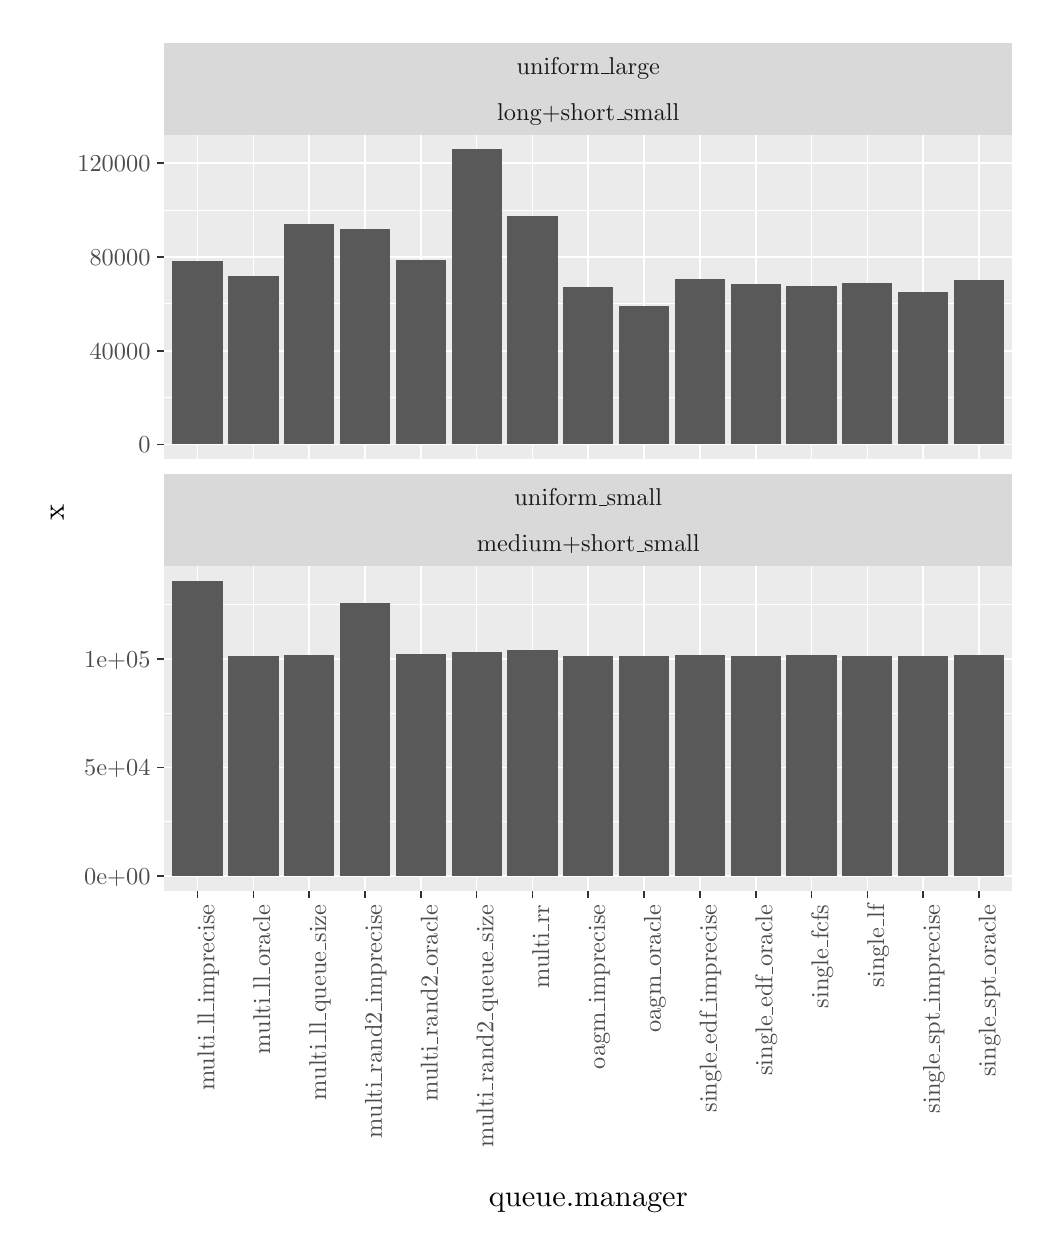
\begin{tikzpicture}[x=1pt,y=1pt]
\definecolor{fillColor}{RGB}{255,255,255}
\path[use as bounding box,fill=fillColor,fill opacity=0.00] (0,0) rectangle (361.35,433.62);
\begin{scope}
\path[clip] (  0.00,  0.00) rectangle (361.35,433.62);
\definecolor{drawColor}{RGB}{255,255,255}
\definecolor{fillColor}{RGB}{255,255,255}

\path[draw=drawColor,line width= 0.6pt,line join=round,line cap=round,fill=fillColor] (  0.00,  0.00) rectangle (361.35,433.62);
\end{scope}
\begin{scope}
\path[clip] ( 49.31,277.67) rectangle (355.85,394.98);
\definecolor{fillColor}{gray}{0.92}

\path[fill=fillColor] ( 49.31,277.67) rectangle (355.85,394.98);
\definecolor{drawColor}{RGB}{255,255,255}

\path[draw=drawColor,line width= 0.3pt,line join=round] ( 49.31,299.94) --
	(355.85,299.94);

\path[draw=drawColor,line width= 0.3pt,line join=round] ( 49.31,333.83) --
	(355.85,333.83);

\path[draw=drawColor,line width= 0.3pt,line join=round] ( 49.31,367.71) --
	(355.85,367.71);

\path[draw=drawColor,line width= 0.6pt,line join=round] ( 49.31,283.00) --
	(355.85,283.00);

\path[draw=drawColor,line width= 0.6pt,line join=round] ( 49.31,316.89) --
	(355.85,316.89);

\path[draw=drawColor,line width= 0.6pt,line join=round] ( 49.31,350.77) --
	(355.85,350.77);

\path[draw=drawColor,line width= 0.6pt,line join=round] ( 49.31,384.66) --
	(355.85,384.66);

\path[draw=drawColor,line width= 0.6pt,line join=round] ( 61.41,277.67) --
	( 61.41,394.98);

\path[draw=drawColor,line width= 0.6pt,line join=round] ( 81.58,277.67) --
	( 81.58,394.98);

\path[draw=drawColor,line width= 0.6pt,line join=round] (101.74,277.67) --
	(101.74,394.98);

\path[draw=drawColor,line width= 0.6pt,line join=round] (121.91,277.67) --
	(121.91,394.98);

\path[draw=drawColor,line width= 0.6pt,line join=round] (142.08,277.67) --
	(142.08,394.98);

\path[draw=drawColor,line width= 0.6pt,line join=round] (162.24,277.67) --
	(162.24,394.98);

\path[draw=drawColor,line width= 0.6pt,line join=round] (182.41,277.67) --
	(182.41,394.98);

\path[draw=drawColor,line width= 0.6pt,line join=round] (202.58,277.67) --
	(202.58,394.98);

\path[draw=drawColor,line width= 0.6pt,line join=round] (222.75,277.67) --
	(222.75,394.98);

\path[draw=drawColor,line width= 0.6pt,line join=round] (242.91,277.67) --
	(242.91,394.98);

\path[draw=drawColor,line width= 0.6pt,line join=round] (263.08,277.67) --
	(263.08,394.98);

\path[draw=drawColor,line width= 0.6pt,line join=round] (283.25,277.67) --
	(283.25,394.98);

\path[draw=drawColor,line width= 0.6pt,line join=round] (303.42,277.67) --
	(303.42,394.98);

\path[draw=drawColor,line width= 0.6pt,line join=round] (323.58,277.67) --
	(323.58,394.98);

\path[draw=drawColor,line width= 0.6pt,line join=round] (343.75,277.67) --
	(343.75,394.98);
\definecolor{fillColor}{gray}{0.35}

\path[fill=fillColor] ( 52.33,283.00) rectangle ( 70.48,349.24);

\path[fill=fillColor] ( 72.50,283.00) rectangle ( 90.65,343.83);

\path[fill=fillColor] ( 92.67,283.00) rectangle (110.82,362.57);

\path[fill=fillColor] (112.83,283.00) rectangle (130.99,361.00);

\path[fill=fillColor] (133.00,283.00) rectangle (151.15,349.78);

\path[fill=fillColor] (153.17,283.00) rectangle (171.32,389.64);

\path[fill=fillColor] (173.34,283.00) rectangle (191.49,365.58);

\path[fill=fillColor] (193.50,283.00) rectangle (211.65,339.88);

\path[fill=fillColor] (213.67,283.00) rectangle (231.82,332.92);

\path[fill=fillColor] (233.84,283.00) rectangle (251.99,342.97);

\path[fill=fillColor] (254.01,283.00) rectangle (272.16,341.08);

\path[fill=fillColor] (274.17,283.00) rectangle (292.32,340.14);

\path[fill=fillColor] (294.34,283.00) rectangle (312.49,341.43);

\path[fill=fillColor] (314.51,283.00) rectangle (332.66,338.12);

\path[fill=fillColor] (334.67,283.00) rectangle (352.82,342.38);
\end{scope}
\begin{scope}
\path[clip] ( 49.31,121.72) rectangle (355.85,239.03);
\definecolor{fillColor}{gray}{0.92}

\path[fill=fillColor] ( 49.31,121.72) rectangle (355.85,239.03);
\definecolor{drawColor}{RGB}{255,255,255}

\path[draw=drawColor,line width= 0.3pt,line join=round] ( 49.31,146.67) --
	(355.85,146.67);

\path[draw=drawColor,line width= 0.3pt,line join=round] ( 49.31,185.92) --
	(355.85,185.92);

\path[draw=drawColor,line width= 0.3pt,line join=round] ( 49.31,225.16) --
	(355.85,225.16);

\path[draw=drawColor,line width= 0.6pt,line join=round] ( 49.31,127.05) --
	(355.85,127.05);

\path[draw=drawColor,line width= 0.6pt,line join=round] ( 49.31,166.30) --
	(355.85,166.30);

\path[draw=drawColor,line width= 0.6pt,line join=round] ( 49.31,205.54) --
	(355.85,205.54);

\path[draw=drawColor,line width= 0.6pt,line join=round] ( 61.41,121.72) --
	( 61.41,239.03);

\path[draw=drawColor,line width= 0.6pt,line join=round] ( 81.58,121.72) --
	( 81.58,239.03);

\path[draw=drawColor,line width= 0.6pt,line join=round] (101.74,121.72) --
	(101.74,239.03);

\path[draw=drawColor,line width= 0.6pt,line join=round] (121.91,121.72) --
	(121.91,239.03);

\path[draw=drawColor,line width= 0.6pt,line join=round] (142.08,121.72) --
	(142.08,239.03);

\path[draw=drawColor,line width= 0.6pt,line join=round] (162.24,121.72) --
	(162.24,239.03);

\path[draw=drawColor,line width= 0.6pt,line join=round] (182.41,121.72) --
	(182.41,239.03);

\path[draw=drawColor,line width= 0.6pt,line join=round] (202.58,121.72) --
	(202.58,239.03);

\path[draw=drawColor,line width= 0.6pt,line join=round] (222.75,121.72) --
	(222.75,239.03);

\path[draw=drawColor,line width= 0.6pt,line join=round] (242.91,121.72) --
	(242.91,239.03);

\path[draw=drawColor,line width= 0.6pt,line join=round] (263.08,121.72) --
	(263.08,239.03);

\path[draw=drawColor,line width= 0.6pt,line join=round] (283.25,121.72) --
	(283.25,239.03);

\path[draw=drawColor,line width= 0.6pt,line join=round] (303.42,121.72) --
	(303.42,239.03);

\path[draw=drawColor,line width= 0.6pt,line join=round] (323.58,121.72) --
	(323.58,239.03);

\path[draw=drawColor,line width= 0.6pt,line join=round] (343.75,121.72) --
	(343.75,239.03);
\definecolor{fillColor}{gray}{0.35}

\path[fill=fillColor] ( 52.33,127.05) rectangle ( 70.48,233.69);

\path[fill=fillColor] ( 72.50,127.05) rectangle ( 90.65,206.70);

\path[fill=fillColor] ( 92.67,127.05) rectangle (110.82,206.80);

\path[fill=fillColor] (112.83,127.05) rectangle (130.99,225.76);

\path[fill=fillColor] (133.00,127.05) rectangle (151.15,207.12);

\path[fill=fillColor] (153.17,127.05) rectangle (171.32,207.95);

\path[fill=fillColor] (173.34,127.05) rectangle (191.49,208.56);

\path[fill=fillColor] (193.50,127.05) rectangle (211.65,206.64);

\path[fill=fillColor] (213.67,127.05) rectangle (231.82,206.63);

\path[fill=fillColor] (233.84,127.05) rectangle (251.99,206.83);

\path[fill=fillColor] (254.01,127.05) rectangle (272.16,206.72);

\path[fill=fillColor] (274.17,127.05) rectangle (292.32,206.87);

\path[fill=fillColor] (294.34,127.05) rectangle (312.49,206.67);

\path[fill=fillColor] (314.51,127.05) rectangle (332.66,206.72);

\path[fill=fillColor] (334.67,127.05) rectangle (352.82,206.78);
\end{scope}
\begin{scope}
\path[clip] ( 49.31,255.60) rectangle (355.85,272.17);
\definecolor{fillColor}{gray}{0.85}

\path[fill=fillColor] ( 49.31,255.60) rectangle (355.85,272.17);
\definecolor{drawColor}{gray}{0.10}

\node[text=drawColor,anchor=base,inner sep=0pt, outer sep=0pt, scale=  0.88] at (202.58,260.85) {uniform\_small};
\end{scope}
\begin{scope}
\path[clip] ( 49.31,239.03) rectangle (355.85,255.60);
\definecolor{fillColor}{gray}{0.85}

\path[fill=fillColor] ( 49.31,239.03) rectangle (355.85,255.60);
\definecolor{drawColor}{gray}{0.10}

\node[text=drawColor,anchor=base,inner sep=0pt, outer sep=0pt, scale=  0.88] at (202.58,244.28) {medium+short\_small};
\end{scope}
\begin{scope}
\path[clip] ( 49.31,411.55) rectangle (355.85,428.12);
\definecolor{fillColor}{gray}{0.85}

\path[fill=fillColor] ( 49.31,411.55) rectangle (355.85,428.12);
\definecolor{drawColor}{gray}{0.10}

\node[text=drawColor,anchor=base,inner sep=0pt, outer sep=0pt, scale=  0.88] at (202.58,416.80) {uniform\_large};
\end{scope}
\begin{scope}
\path[clip] ( 49.31,394.98) rectangle (355.85,411.55);
\definecolor{fillColor}{gray}{0.85}

\path[fill=fillColor] ( 49.31,394.98) rectangle (355.85,411.55);
\definecolor{drawColor}{gray}{0.10}

\node[text=drawColor,anchor=base,inner sep=0pt, outer sep=0pt, scale=  0.88] at (202.58,400.23) {long+short\_small};
\end{scope}
\begin{scope}
\path[clip] (  0.00,  0.00) rectangle (361.35,433.62);
\definecolor{drawColor}{gray}{0.20}

\path[draw=drawColor,line width= 0.6pt,line join=round] ( 61.41,118.97) --
	( 61.41,121.72);

\path[draw=drawColor,line width= 0.6pt,line join=round] ( 81.58,118.97) --
	( 81.58,121.72);

\path[draw=drawColor,line width= 0.6pt,line join=round] (101.74,118.97) --
	(101.74,121.72);

\path[draw=drawColor,line width= 0.6pt,line join=round] (121.91,118.97) --
	(121.91,121.72);

\path[draw=drawColor,line width= 0.6pt,line join=round] (142.08,118.97) --
	(142.08,121.72);

\path[draw=drawColor,line width= 0.6pt,line join=round] (162.24,118.97) --
	(162.24,121.72);

\path[draw=drawColor,line width= 0.6pt,line join=round] (182.41,118.97) --
	(182.41,121.72);

\path[draw=drawColor,line width= 0.6pt,line join=round] (202.58,118.97) --
	(202.58,121.72);

\path[draw=drawColor,line width= 0.6pt,line join=round] (222.75,118.97) --
	(222.75,121.72);

\path[draw=drawColor,line width= 0.6pt,line join=round] (242.91,118.97) --
	(242.91,121.72);

\path[draw=drawColor,line width= 0.6pt,line join=round] (263.08,118.97) --
	(263.08,121.72);

\path[draw=drawColor,line width= 0.6pt,line join=round] (283.25,118.97) --
	(283.25,121.72);

\path[draw=drawColor,line width= 0.6pt,line join=round] (303.42,118.97) --
	(303.42,121.72);

\path[draw=drawColor,line width= 0.6pt,line join=round] (323.58,118.97) --
	(323.58,121.72);

\path[draw=drawColor,line width= 0.6pt,line join=round] (343.75,118.97) --
	(343.75,121.72);
\end{scope}
\begin{scope}
\path[clip] (  0.00,  0.00) rectangle (361.35,433.62);
\definecolor{drawColor}{gray}{0.30}

\node[text=drawColor,rotate= 90.00,anchor=base east,inner sep=0pt, outer sep=0pt, scale=  0.88] at ( 67.47,116.77) {multi\_ll\_imprecise};

\node[text=drawColor,rotate= 90.00,anchor=base east,inner sep=0pt, outer sep=0pt, scale=  0.88] at ( 87.64,116.77) {multi\_ll\_oracle};

\node[text=drawColor,rotate= 90.00,anchor=base east,inner sep=0pt, outer sep=0pt, scale=  0.88] at (107.80,116.77) {multi\_ll\_queue\_size};

\node[text=drawColor,rotate= 90.00,anchor=base east,inner sep=0pt, outer sep=0pt, scale=  0.88] at (127.97,116.77) {multi\_rand2\_imprecise};

\node[text=drawColor,rotate= 90.00,anchor=base east,inner sep=0pt, outer sep=0pt, scale=  0.88] at (148.14,116.77) {multi\_rand2\_oracle};

\node[text=drawColor,rotate= 90.00,anchor=base east,inner sep=0pt, outer sep=0pt, scale=  0.88] at (168.31,116.77) {multi\_rand2\_queue\_size};

\node[text=drawColor,rotate= 90.00,anchor=base east,inner sep=0pt, outer sep=0pt, scale=  0.88] at (188.47,116.77) {multi\_rr};

\node[text=drawColor,rotate= 90.00,anchor=base east,inner sep=0pt, outer sep=0pt, scale=  0.88] at (208.64,116.77) {oagm\_imprecise};

\node[text=drawColor,rotate= 90.00,anchor=base east,inner sep=0pt, outer sep=0pt, scale=  0.88] at (228.81,116.77) {oagm\_oracle};

\node[text=drawColor,rotate= 90.00,anchor=base east,inner sep=0pt, outer sep=0pt, scale=  0.88] at (248.97,116.77) {single\_edf\_imprecise};

\node[text=drawColor,rotate= 90.00,anchor=base east,inner sep=0pt, outer sep=0pt, scale=  0.88] at (269.14,116.77) {single\_edf\_oracle};

\node[text=drawColor,rotate= 90.00,anchor=base east,inner sep=0pt, outer sep=0pt, scale=  0.88] at (289.31,116.77) {single\_fcfs};

\node[text=drawColor,rotate= 90.00,anchor=base east,inner sep=0pt, outer sep=0pt, scale=  0.88] at (309.48,116.77) {single\_lf};

\node[text=drawColor,rotate= 90.00,anchor=base east,inner sep=0pt, outer sep=0pt, scale=  0.88] at (329.64,116.77) {single\_spt\_imprecise};

\node[text=drawColor,rotate= 90.00,anchor=base east,inner sep=0pt, outer sep=0pt, scale=  0.88] at (349.81,116.77) {single\_spt\_oracle};
\end{scope}
\begin{scope}
\path[clip] (  0.00,  0.00) rectangle (361.35,433.62);
\definecolor{drawColor}{gray}{0.30}

\node[text=drawColor,anchor=base east,inner sep=0pt, outer sep=0pt, scale=  0.88] at ( 44.36,279.97) {0};

\node[text=drawColor,anchor=base east,inner sep=0pt, outer sep=0pt, scale=  0.88] at ( 44.36,313.86) {40000};

\node[text=drawColor,anchor=base east,inner sep=0pt, outer sep=0pt, scale=  0.88] at ( 44.36,347.74) {80000};

\node[text=drawColor,anchor=base east,inner sep=0pt, outer sep=0pt, scale=  0.88] at ( 44.36,381.63) {120000};
\end{scope}
\begin{scope}
\path[clip] (  0.00,  0.00) rectangle (361.35,433.62);
\definecolor{drawColor}{gray}{0.20}

\path[draw=drawColor,line width= 0.6pt,line join=round] ( 46.56,283.00) --
	( 49.31,283.00);

\path[draw=drawColor,line width= 0.6pt,line join=round] ( 46.56,316.89) --
	( 49.31,316.89);

\path[draw=drawColor,line width= 0.6pt,line join=round] ( 46.56,350.77) --
	( 49.31,350.77);

\path[draw=drawColor,line width= 0.6pt,line join=round] ( 46.56,384.66) --
	( 49.31,384.66);
\end{scope}
\begin{scope}
\path[clip] (  0.00,  0.00) rectangle (361.35,433.62);
\definecolor{drawColor}{gray}{0.30}

\node[text=drawColor,anchor=base east,inner sep=0pt, outer sep=0pt, scale=  0.88] at ( 44.36,124.02) {0e+00};

\node[text=drawColor,anchor=base east,inner sep=0pt, outer sep=0pt, scale=  0.88] at ( 44.36,163.27) {5e+04};

\node[text=drawColor,anchor=base east,inner sep=0pt, outer sep=0pt, scale=  0.88] at ( 44.36,202.51) {1e+05};
\end{scope}
\begin{scope}
\path[clip] (  0.00,  0.00) rectangle (361.35,433.62);
\definecolor{drawColor}{gray}{0.20}

\path[draw=drawColor,line width= 0.6pt,line join=round] ( 46.56,127.05) --
	( 49.31,127.05);

\path[draw=drawColor,line width= 0.6pt,line join=round] ( 46.56,166.30) --
	( 49.31,166.30);

\path[draw=drawColor,line width= 0.6pt,line join=round] ( 46.56,205.54) --
	( 49.31,205.54);
\end{scope}
\begin{scope}
\path[clip] (  0.00,  0.00) rectangle (361.35,433.62);
\definecolor{drawColor}{RGB}{0,0,0}

\node[text=drawColor,anchor=base,inner sep=0pt, outer sep=0pt, scale=  1.10] at (202.58,  7.64) {queue.manager};
\end{scope}
\begin{scope}
\path[clip] (  0.00,  0.00) rectangle (361.35,433.62);
\definecolor{drawColor}{RGB}{0,0,0}

\node[text=drawColor,rotate= 90.00,anchor=base,inner sep=0pt, outer sep=0pt, scale=  1.10] at ( 13.08,258.35) {x};
\end{scope}
\end{tikzpicture}
